
\documentclass[letterpaper,hide notes,xcolor={table,svgnames},pdftex]{beamer}
\def\showexamples{t}


%\usepackage[svgnames]{xcolor}

%% Demo talk
%\documentclass[letterpaper,notes=show]{beamer}

\usecolortheme{crane}
\setbeamertemplate{navigation symbols}{}

\usetheme{MyPittsburgh}
%\usetheme{Frankfurt}

%\usepackage{tipa}

\usepackage{hyperref}
\usepackage{graphicx,xspace}
\usepackage[normalem]{ulem}

\newcommand\SF[1]{$\bigstar$\footnote{SF: #1}}



\newcounter{tmpnumSlide}
\newcounter{tmpnumNote}

% old question code
%\newcommand\question[1]{{$\bigstar$ \small \onlySlide{2}{#1}}}
% \newcommand\nquestion[1]{\ifdefined \presentationonly \textcircled{?} \fi \note{\par{\Large \textbf{?}} #1}}
% \newcommand\nanswer[1]{\note{\par{\Large \textbf{A}} #1}}


 \newcommand\mnote[1]{%
   \addtocounter{tmpnumSlide}{1}
   \ifdefined\showcues {~\tiny\fbox{\arabic{tmpnumSlide}}}\fi
   \note{\setlength{\parskip}{1ex}\addtocounter{tmpnumNote}{1}\textbf{\Large \arabic{tmpnumNote}:} {#1\par}}}

\newcommand\mmnote[1]{\note{\setlength{\parskip}{1ex}#1\par}}

%\newcommand\mnote[2][]{\ifdefined\handoutwithnotes {~\tiny\fbox{#1}}\fi
% \note{\setlength{\parskip}{1ex}\textbf{\Large #1:} #2\par}}

%\newcommand\mnote[2][]{{\tiny\fbox{#1}} \note{\setlength{\parskip}{1ex}\textbf{\Large #1:} #2\par}}

\newcommand\mquestion[2]{{~\color{red}\fbox{?}}\note{\setlength{\parskip}{1ex}\par{\Large \textbf{?}} #1} \note{\setlength{\parskip}{1ex}\par{\Large \textbf{A}} #2\par}\ifdefined \presentationonly \pause \fi}

\newcommand\blackboard[1]{%
\ifdefined   \showblackboard
  {#1}
  \else {\begin{center} \fbox{\colorbox{blue!30}{%
         \begin{minipage}{.95\linewidth}%
           \hspace{\stretch{1}} Some space intentionally left blank; done at the blackboard.%
         \end{minipage}}}\end{center}}%
         \fi%
}



%\newcommand\q{\tikz \node[thick,color=black,shape=circle]{?};}
%\newcommand\q{\ifdefined \presentationonly \textcircled{?} \fi}

\usepackage{listings}
\lstset{%
  keywordstyle=\bfseries,
  aboveskip=15pt,
  belowskip=15pt,
  captionpos=b,
  identifierstyle=\ttfamily,
  escapeinside={(*@}{@*)},
  stringstyle=\ttfamiliy,
  frame=lines,
  numbers=left, basicstyle=\scriptsize, numberstyle=\tiny, stepnumber=0, numbersep=2pt}

\usepackage{siunitx}
\newcommand\sius[1]{\num[group-separator = {,}]{#1}\si{\micro\second}}
\newcommand\sims[1]{\num[group-separator = {,}]{#1}\si{\milli\second}}
\newcommand\sins[1]{\num[group-separator = {,}]{#1}\si{\nano\second}}
\sisetup{group-separator = {,}, group-digits = true}

%% -------------------- tikz --------------------
\usepackage{tikz}
\usetikzlibrary{positioning}
\usetikzlibrary{arrows,backgrounds,automata,decorations.shapes,decorations.pathmorphing,decorations.markings,decorations.text}

\tikzstyle{place}=[circle,draw=blue!50,fill=blue!20,thick, inner sep=0pt,minimum size=6mm]
\tikzstyle{transition}=[rectangle,draw=black!50,fill=black!20,thick, inner sep=0pt,minimum size=4mm]

\tikzstyle{block}=[rectangle,draw=black, thick, inner sep=5pt]
\tikzstyle{bullet}=[circle,draw=black, fill=black, thin, inner sep=2pt]

\tikzstyle{pre}=[<-,shorten <=1pt,>=stealth',semithick]
\tikzstyle{post}=[->,shorten >=1pt,>=stealth',semithick]
\tikzstyle{bi}=[<->,shorten >=1pt,shorten <=1pt, >=stealth',semithick]

\tikzstyle{mut}=[-,>=stealth',semithick]

\tikzstyle{treereset}=[dashed,->, shorten >=1pt,>=stealth',thin]

\usepackage{ifmtarg}
\usepackage{xifthen}
\makeatletter
% new counter to now which frame it is within the sequence
\newcounter{multiframecounter}
% initialize buffer for previously used frame title
\gdef\lastframetitle{\textit{undefined}}
% new environment for a multi-frame
\newenvironment{multiframe}[1][]{%
\ifthenelse{\isempty{#1}}{%
% if no frame title was set via optional parameter,
% only increase sequence counter by 1
\addtocounter{multiframecounter}{1}%
}{%
% new frame title has been provided, thus
% reset sequence counter to 1 and buffer frame title for later use
\setcounter{multiframecounter}{1}%
\gdef\lastframetitle{#1}%
}%
% start conventional frame environment and
% automatically set frame title followed by sequence counter
\begin{frame}%
\frametitle{\lastframetitle~{\normalfont(\arabic{multiframecounter})}}%
}{%
\end{frame}%
}
\makeatother

\makeatletter
\newdimen\tu@tmpa%
\newdimen\ydiffl%
\newdimen\xdiffl%
\newcommand\ydiff[2]{%
    \coordinate (tmpnamea) at (#1);%
    \coordinate (tmpnameb) at (#2);%
    \pgfextracty{\tu@tmpa}{\pgfpointanchor{tmpnamea}{center}}%
    \pgfextracty{\ydiffl}{\pgfpointanchor{tmpnameb}{center}}%
    \advance\ydiffl by -\tu@tmpa%
}
\newcommand\xdiff[2]{%
    \coordinate (tmpnamea) at (#1);%
    \coordinate (tmpnameb) at (#2);%
    \pgfextractx{\tu@tmpa}{\pgfpointanchor{tmpnamea}{center}}%
    \pgfextractx{\xdiffl}{\pgfpointanchor{tmpnameb}{center}}%
    \advance\xdiffl by -\tu@tmpa%
}
\makeatother
\newcommand{\copyrightbox}[3][r]{%
\begin{tikzpicture}%
\node[inner sep=0pt,minimum size=2em](ciimage){#2};
\usefont{OT1}{phv}{n}{n}\fontsize{4}{4}\selectfont
\ydiff{ciimage.south}{ciimage.north}
\xdiff{ciimage.west}{ciimage.east}
\ifthenelse{\equal{#1}{r}}{%
\node[inner sep=0pt,right=1ex of ciimage.south east,anchor=north west,rotate=90]%
{\raggedleft\color{black!50}\parbox{\the\ydiffl}{\raggedright{}#3}};%
}{%
\ifthenelse{\equal{#1}{l}}{%
\node[inner sep=0pt,right=1ex of ciimage.south west,anchor=south west,rotate=90]%
{\raggedleft\color{black!50}\parbox{\the\ydiffl}{\raggedright{}#3}};%
}{%
\node[inner sep=0pt,below=1ex of ciimage.south west,anchor=north west]%
{\raggedleft\color{black!50}\parbox{\the\xdiffl}{\raggedright{}#3}};%
}
}
\end{tikzpicture}
}


%% --------------------

%\usepackage[excludeor]{everyhook}
%\PushPreHook{par}{\setbox0=\lastbox\llap{MUH}}\box0}

%\vspace*{\stretch{1}

%\setbox0=\lastbox \llap{\textbullet\enskip}\box0}

\setlength{\parskip}{\fill}

\newcommand\noskips{\setlength{\parskip}{1ex}}
\newcommand\doskips{\setlength{\parskip}{\fill}}

\newcommand\xx{\par\vspace*{\stretch{1}}\par}
\newcommand\xxs{\par\vspace*{2ex}\par}
\newcommand\tuple[1]{\langle #1 \rangle}
\newcommand\code[1]{{\sf \footnotesize #1}}
\newcommand\ex[1]{\uline{Example:} \ifdefined \presentationonly \pause \fi
  \ifdefined\showexamples#1\xspace\else{\uline{\hspace*{2cm}}}\fi}

\newcommand\ceil[1]{\lceil #1 \rceil}


\AtBeginSection[]
{
   \begin{frame}
       \frametitle{Outline}
       \tableofcontents[currentsection]
   \end{frame}
}



\pgfdeclarelayer{edgelayer}
\pgfdeclarelayer{nodelayer}
\pgfsetlayers{edgelayer,nodelayer,main}

\tikzstyle{none}=[inner sep=0pt]
\tikzstyle{rn}=[circle,fill=Red,draw=Black,line width=0.8 pt]
\tikzstyle{gn}=[circle,fill=Lime,draw=Black,line width=0.8 pt]
\tikzstyle{yn}=[circle,fill=Yellow,draw=Black,line width=0.8 pt]
\tikzstyle{empty}=[circle,fill=White,draw=Black]
\tikzstyle{bw} = [rectangle, draw, fill=blue!20, 
    text width=4em, text centered, rounded corners, minimum height=2em]
    
    \newcommand{\CcNote}[1]{% longname
	This work is licensed under the \textit{Creative Commons #1 3.0 License}.%
}
\newcommand{\CcImageBy}[1]{%
	\includegraphics[scale=#1]{creative_commons/cc_by_30.pdf}%
}
\newcommand{\CcImageSa}[1]{%
	\includegraphics[scale=#1]{creative_commons/cc_sa_30.pdf}%
}
\newcommand{\CcImageNc}[1]{%
	\includegraphics[scale=#1]{creative_commons/cc_nc_30.pdf}%
}
\newcommand{\CcGroupBySa}[2]{% zoom, gap
	\CcImageBy{#1}\hspace*{#2}\CcImageNc{#1}\hspace*{#2}\CcImageSa{#1}%
}
\newcommand{\CcLongnameByNcSa}{Attribution-NonCommercial-ShareAlike}

\newenvironment{changemargin}[1]{% 
  \begin{list}{}{% 
    \setlength{\topsep}{0pt}% 
    \setlength{\leftmargin}{#1}% 
    \setlength{\rightmargin}{1em}
    \setlength{\listparindent}{\parindent}% 
    \setlength{\itemindent}{\parindent}% 
    \setlength{\parsep}{\parskip}% 
  }% 
  \item[]}{\end{list}} 




\title{Lecture 21 --- Planning}

\author{Patrick Lam \\ \small \texttt{p.lam@ece.uwaterloo.ca}}
\institute{Department of Electrical and Computer Engineering \\[-1ex]
  University of Waterloo}
\date{\today}


\begin{document}

\begin{frame}
  \titlepage
\end{frame}


\begin{frame}
\frametitle{Planning, scheduling, and estimation}

\begin{changemargin}{1cm}
Planning and scheduling are notoriously difficult, because estimates
are often wrong.

\begin{itemize}
\item {\bf Planning.} Given a project, figure out \alert{how} to do the
project. Figure out subtasks.\\[1em]
\item {\bf Scheduling.} Assign \alert{start} and \alert{end times} to subtasks. More mechanical. \\[1em]
\item {\bf Estimation.} Informed guess (based on facts) about \alert{resources
needed} to accomplish a task. \\ Used in scheduling.
\end{itemize}
\end{changemargin}

\end{frame}

\part{Planning}
\frame{\partpage}


\begin{frame}
\frametitle{Documents}

\Large
\begin{changemargin}{1cm}
\begin{itemize}
\item {\bf Vision and Scope Document}: \\ \qquad preliminary document.
\item {\bf Project Plan}: \\ \qquad  contains all the details.
\end{itemize}
\end{changemargin}

\end{frame}

\begin{frame}
\frametitle{Vision and Scope Document}

\begin{changemargin}{1cm}

Preliminary requirements gathering: \\
make sure that all stakeholders
are on board. \\[1em]

A {\bf vision and scope document} summarizes the design problem, the
stakeholders, the users, the risks, the assumptions, and the desired
features of a solution. 
\end{changemargin}

\end{frame}

\begin{frame}

\frametitle{Goals of a Vision and Scope Document}

\large
\begin{changemargin}{1cm}
A vision and scope document:
\begin{itemize}
\item identifies \alert{included} features;
\item discusses features that are \alert{out-of-scope};
\item \alert{summarizes} agreed-upon expectations about scope.
\end{itemize}
\end{changemargin}

\end{frame}

\begin{frame}
\frametitle{Vision and Scope Document Outline}

\begin{changemargin}{1cm}
Mousetrap Example
\begin{itemize}
\item Problem Statement \mnote{The project will develop a research prototype for a
better mousetrap.}
\item Project Background \mnote{[Some paragraphs briefly discussing the
  current state of the art in mousetrap design.]}
\item Stakeholders \mnote{The ACME Corporation eventually aims to sell these
  mousetraps to end users.}
\item Users \mnote{ End users will deploy the mousetraps in mouse-infested
  locations.}
\item Risks \mnote{Mousetrap technology is a mature area, and many inventors
  have already attempted to develop better mousetraps, so this project
  may not successfully invent a better mousetrap.}
\item Assumptions \mnote{The engineers have access to modern CAD software, a
  machine shop, and commonplace electronic components, for building
  their better mousetrap. The engineers' toy mice accurately represent
  the behaviour of actual real-world mice.}
\item Vision of the Solution \mnote{The better mousetrap will use modern
  embedded systems technology, including sensors and actuators, to 
  effectively detect and trap mice without harming them.}
\item List of features \mnote{The mousetrap will be able to detect and capture
  mice. Users will be able to calibrate the mousetrap for their intended
  deployment area. The mousetrap will include a provision for including 
  mousebait.}
\item Scope of phased release \mnote{The first version of the mousetrap will
  detect mice, but will not capture the mice. The second version will
  detect and capture mice.}
\item Features not to be developed \mnote{It remains the responsibility of the
  end-user to relocate the mice that this mousetrap catches.}
\end{itemize}
\end{changemargin}

\end{frame}

\begin{frame}
\frametitle{Project Plan}

\begin{changemargin}{1cm}
The project plan breaks down\\ \alert{what} to do and
\alert{who} is to do it.

\begin{itemize}
\item Statement of Work: what to do and who will do it.
\item Resource List: who can do it, and with what.
\item Work Breakdown Structure: what to do (more detail).
\item Project Schedule: when to do it.
\item Risk Plan: what might go wrong.
\end{itemize}

We'll look at each part of the project plan.
\end{changemargin}

\end{frame}

\begin{frame}
\frametitle{Statement of Work}

\begin{changemargin}{1cm}
A {\bf statement of work} (SOW) describes all work products to be
produced and identifies who will do the work, including:

\begin{itemize}
\item a list of \alert{all project features} that will be developed;
\item a \alert{description} of each deliverable that will be developed \\ (at
  this stage, one paragraph per deliverable); and
\item the \alert{estimated effort} required for each deliverable, if known.
\end{itemize}
\end{changemargin}

\end{frame}

\begin{frame}
\frametitle{Resource List}

\begin{changemargin}{1cm}

\begin{itemize}
\item {\bf Resource List}: enumerates all resources required for the
project and summarizes the availability of the resources.

\item {\bf Resource}: person, hardware component, software
licence, room, or anything else necessary for the project
but limited in availability.
\end{itemize}
\end{changemargin}

\end{frame}

\begin{frame}
\frametitle{Components of Resource List}

\begin{changemargin}{1cm}

The resource list has the following components:
\begin{itemize}
\item resource name;
\item brief (one-line) description of the resource; 
\item resource availability (e.g. start dates, end dates);
\item cost of the resource (if applicable).
\end{itemize}

\end{changemargin}

\end{frame}

\begin{frame}
\frametitle{Work Breakdown Structure (WBS)}

\begin{changemargin}{1cm}
A {\bf work breakdown structure} (WBS) describes all project
activities:

\begin{itemize}
\item comprehensively lists all project activities
required to complete the project;\\

(includes intermediate deliverables.)

\item must evolve with your understanding of the project;

\item should be kept in a revision control repository.
\end{itemize}

\emph{Applied Software Project Management} describes the
``Wideband Delphi Process'' for estimating the time required for each
activity in a WBS.
\end{changemargin}

\end{frame}

\begin{frame}

\frametitle{Project Schedule}

\begin{changemargin}{1cm}

A {\bf project schedule} estimates start \& end times for project
activities. 

One way of getting estimates: run a meeting.
\begin{enumerate}
\item Each participant writes down an initial estimate \\ plus assumptions.
\item Moderator collects all estimates and summarizes them.
\item Participants discuss the estimates.
\item Repeat as needed.
\end{enumerate}

~\\

Documenting assumptions helps refine estimates and\\  reduce variance in
estimates. 

\end{changemargin}
\end{frame}

\begin{frame}
\frametitle{Risk Plan}

\begin{changemargin}{1cm}


A {\bf risk} is a potential threat to the successful completion
of your project. \\[1em]

A {\bf risk plan} describes:
\begin{itemize}
\item anticipated risks;
\item the likelihood of their occurrence; and
\item how to mitigate these risks.
\end{itemize}

Good risk plans are comprehensive and include potential ways to
mitigate significant risks.

\end{changemargin}

\end{frame}

\begin{frame}
\frametitle{Developing a Risk Plan}

\begin{changemargin}{1cm}

The risk plan is usually developed in a risk assessment and planning session.
Team members:
\begin{itemize}
\item \alert{brainstorm} to list potential risks;
\item \alert{estimate} likelihood of each risk and its impact;
\item \alert{develop} a plan for mitigating likely and severe risks.
\end{itemize}

~\\

\end{changemargin}

\end{frame}

\part{Estimation}
\frame{\partpage}

\begin{frame}
\frametitle{Estimates}

\begin{changemargin}{1cm}

\emph{Plans} include \emph{schedules}, which rely on \alert{estimates}.\\[1em]

Estimates often get overrun\\ (why? because you make best-case assumptions).\\[1em]

Prerequisites for good estimates:
\begin{itemize}
\item an accurate work breakdown structure;
\item an effort estimate for each task in the WBS;
\item a list of assumptions behind the estimates; and
\item consensus that estimates are reasonable.
\end{itemize}

\end{changemargin}

\end{frame}


\begin{frame}
\frametitle{Assumptions in Estimates}

\begin{changemargin}{1cm}

Do assumptions make estimates less accurate? \\
\hspace*{3em}\alert{Not necessarily!}\\
Unstated assumptions, however, are troublesome.\\[1em]

If an assumption is well-documented and properly communicated, it can
improve the quality of an estimate, by:
\begin{itemize}
\item revealing an inobvious problem or detail; or,
\item revealing a simplification that some, but not all, members of the estimation team were relying on.
\end{itemize}


Finding out that an assumption is untrue is a good time to revisit an estimate.\\[1em]

Agreeing on assumptions allows estimators to
move beyond the assumptions and come up with good estimates.

\end{changemargin}
\end{frame}


\begin{frame}
\frametitle{Padding Estimates}

\begin{center}

\includegraphics[width=.75\textwidth]{images/scotty.jpg}
\end{center}

\end{frame}

\begin{frame}
\frametitle{Padding Estimates}

\begin{changemargin}{1cm}

(``Scotty Time\footnote{\url{http://tvtropes.org/pmwiki/pmwiki.php/Main/ScottyTime}}''). Padding an estimate seems like all win: underpromise and overdeliver, etc. \\[1em]

% 14:55 at http://www.youtube.com/watch?v=LdShpVwQr9s

Pros:
\begin{itemize}
\item Look like a hero.
\item Less time pressure.
\end{itemize}

Cons:
\begin{itemize}
\item Managers aren't dumb.
\item Clients/managers may decide to not proceed based on padded estimate.
\end{itemize}

\end{changemargin}
\end{frame}

\begin{frame}

\frametitle{Estimation Techniques}

\large
\begin{changemargin}{1cm}

Some estimation techniques:

\begin{itemize}
\item Wideband Delphi
\item PROBE
\item COCOMO II
\item The Planning Game
\end{itemize}

\end{changemargin}
\end{frame}

\begin{frame}
\frametitle{Steps in Wideband Delphi Process}

\begin{changemargin}{1cm}

Straightforward steps:
\begin{itemize}
\item Choose team and moderator.
\item Kickoff meeting: WBS, assumptions, unit of estimation.
\item Team members independently prepare estimates and more assumptions.
\item Estimation session: the moderator
\begin{enumerate}
\item requests estimates;
\item attempts to achieve consensus by having members explain their estimates.
\end{enumerate}
\item Assemble the final list of tasks and estimates.
\item Review results with project manager and team.
\end{itemize}
Estimation sessions are key to the Wideband Delphi Process.
\end{changemargin}

\end{frame}

\begin{frame}
\frametitle{Running an Estimation Session}

\begin{changemargin}{1cm}

\begin{enumerate}
\item Team members share effort estimates for each WBS task.
\item Moderator records estimates and plots
them on a graph or records them in a table. 
\end{enumerate}

Estimates can range widely, because team members may make different
assumptions. 
\end{changemargin}

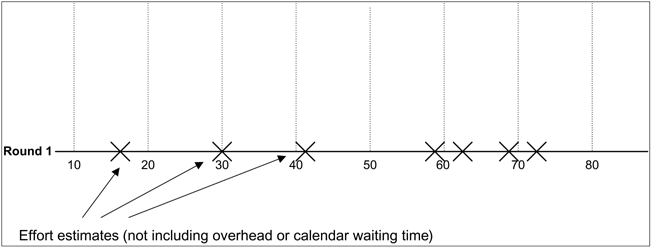
\includegraphics[width=\textwidth]{images/effort-estimates.png}

\end{frame}

\begin{frame}
\frametitle{Achieving Consensus}

\begin{changemargin}{1cm}

Point of working in a team: do better than individuals would.\\[1em]

Wideband Delphi: multiple rounds of discussion.\\[1em]

In each round, team members discuss assumptions,\\ clarify
project details, and revise estimates. \\[1em]

Here's an example of convergence
in estimates:
\end{changemargin}
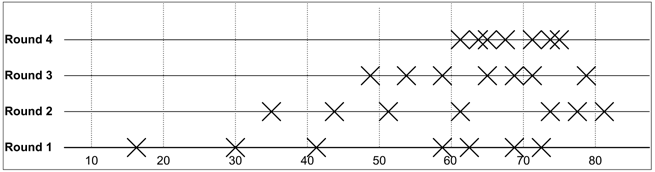
\includegraphics[width=\textwidth]{images/converging-effort-estimates.png}

\end{frame}

\begin{frame}
\frametitle{Other Estimation Techniques: PROBE}

\begin{changemargin}{.75cm}

Idea: Doing something again should take\\ about as long as it did last time.\\[1em]

Obsessively track how long it took to do things in the past, then
use linear regression to estimate how long it'll take in the future.\\[1em]

There are some problems with this approach, though.
% killer overhead, doesn't necessarily generalize, 
% doesn't work well for newbies.
\end{changemargin}
\end{frame}

\begin{frame}
\frametitle{Other Estimation Techniques: COCOMO II}

\begin{changemargin}{1cm}

Idea: Feed in guesses about project's scope, apply a formula, get
estimate of size and effort.\\[1em]

The formula is full of fudge factors (from empirical data).\\[1em]

Examples of inputs: 
\begin{itemize}
\item Memory constraints
\item Analyst capability
\item Product complexity
\end{itemize}

~\\

COCOMO stands for
\emph{COnstructive COst MOdel}.
\end{changemargin}

\end{frame}

\begin{frame}
\frametitle{Other Estimation Techniques: The Planning Game}

\begin{changemargin}{1cm}

Not this kind of game:

\begin{center}

\includegraphics[width=0.5\textwidth]{images/killzone3.jpg}
\end{center}
\end{changemargin}

\end{frame}

\begin{frame}

\frametitle{The Planning Game: Description}

\begin{changemargin}{1cm}
Instead: an estimation technique developed by \\ Kent Beck (inventor of
extreme programming) \\ while working at Chrysler in the 1990's.\\[1em]

The Planning Game is a full planning process that:
\begin{enumerate}
\item identifies the scope of the project;
\item identifies tasks required to complete the project; and
\item estimates the effort required for these tasks.
\end{enumerate}
\end{changemargin}
\end{frame}

\begin{frame}

\frametitle{The Planning Game: Phases}

\begin{changemargin}{1cm}

Two phases: 
\begin{itemize}
\item Release planning---plans the scope of the project.
\item Iteration planning---plans the activities and tasks of the developers.
\end{itemize}

The Planning Game requires a team consisting of customers and developers.

\end{changemargin}
\end{frame}

\begin{frame}

\frametitle{The Planning Game: Phases}

\begin{changemargin}{1cm}

Each week, \\team meets to plan the immediate future of the project:

\begin{itemize}
\item writes user stories\\ describing project requirements on index cards;
\item assigns effort estimates for the stories \\ (e.g., 1, 2, or 3 weeks); and
\item prioritizes the requirements.
\end{itemize}

\end{changemargin}
\end{frame}

\begin{frame}

\frametitle{The Planning Game: Iteration Planning}

\begin{changemargin}{1cm}

Occasionally, the team:

\begin{itemize}
\item divides requirements into sets of tasks to be completed;
\item assigns these tasks to developers; and,
\item estimates effort for these tasks.
\end{itemize}

Developers complete tasks and\\ match them with the user
stories.
\end{changemargin}

\end{frame}

\end{document}
